\documentclass{article}
\usepackage{graphicx}
\usepackage{hyperref}
\usepackage{caption}
\usepackage{subcaption}
\usepackage{mathtools}
\usepackage[dutch]{babel}

\begin{document}

\begin{center}
	\huge{Wiskunde in Kunst}\\
	\LARGE{Opdracht 11} \\
	
	\vspace{2cm}
	
	\Large{Wiskunde kunstwerk}\\
	
	\vfill
	
	\begin{figure}[Hh]
		\centering
		
\includegraphics[width=\textwidth]{tesselation.png}
	\end{figure}
	
	\vfill
	\Large{Marcelo Dias Avelino} \hfill \large{0840416}
\end{center}

\thispagestyle{empty} % Remove page numbering

\pagebreak

\setcounter{page}{1} % Start counting pages here

\section{Hoe is het gemaakt?}

Het kunstwerk gemaakt de deze opdracht is gebaseerd op tessellatie. Dit betekent dat het uit een basis `stukje' bestaat en door deze meerdere keren rondom elkaar te plakken ontstaat er een behangpatroon. De gemaakte stappen om tot dit kunstwerk te komen zijn afgebeeld in Figuur \ref{fig:tesselatie}. Zoals afgebeeld in  Figuur \ref{fig:stap1} en \ref{fig:stap2}, de eerste stap is om een vierkant te tekenen en uit deze vierkant aan \'e\'en van de zijdes een zelf te kiezen gebied af te knippen en vervolgens aan te tegenover gestelde zijde te plakken. Voor dit kunstwerk is er gekozen om een extra zijde te knippen en over te plakken, in dit geval de vorm die te zien is op Figuur \ref{fig:stap3} en \ref{fig:stap4}. Nadat de definitief vorm is gecreëerd, moet er een tweede kleur worden gekozen om de patroon te vormen. Er is voor zwart gekozen in dit kunstwerk en op Figuur \ref{fig:stap5} is er te zien hoe dit eruit ziet. Als de nieuwe kleur gekozen is valt er alleen maar te kopi\"eren en plakken totdat het hele doek vol is behangen zoals gedaan wordt op Figuur \ref{fig:stap6} en zal uiteindelijk uitkomen op het finale versie die te zien is op de voorpagina.

\begin{figure}[Hh]
	\centering
	\begin{subfigure}[b]{0.3\textwidth}    
        
\includegraphics[width=\textwidth]{piece1.png}
        \caption{Stap 1.}
        \label{fig:stap1}
    \end{subfigure}%
    ~
    \begin{subfigure}[b]{0.3\textwidth}    
        
\includegraphics[width=\textwidth]{piece2.png}
        \caption{Stap 2.}
        \label{fig:stap2}
    \end{subfigure}%
    ~
    \begin{subfigure}[b]{0.3\textwidth}    
        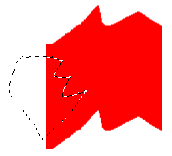
\includegraphics[width=\textwidth]{piece3.png}
        \caption{Stap 3.}
        \label{fig:stap3}
    \end{subfigure}%

    \begin{subfigure}[b]{0.3\textwidth}    
        
\includegraphics[width=\textwidth]{piece4.png}
        \caption{Stap 4.}
        \label{fig:stap4}
    \end{subfigure}%
     ~
    \begin{subfigure}[b]{0.3\textwidth}    
        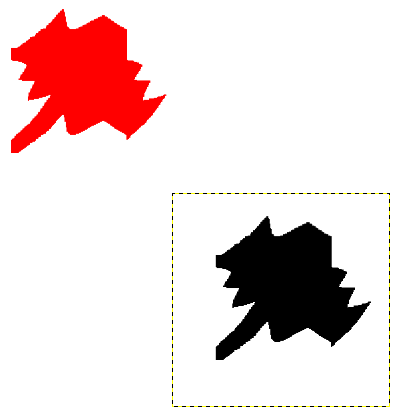
\includegraphics[width=\textwidth]{piece5.png}
        \caption{Stap 5.}
        \label{fig:stap5}
    \end{subfigure}%
     ~
    \begin{subfigure}[b]{0.3\textwidth}    
        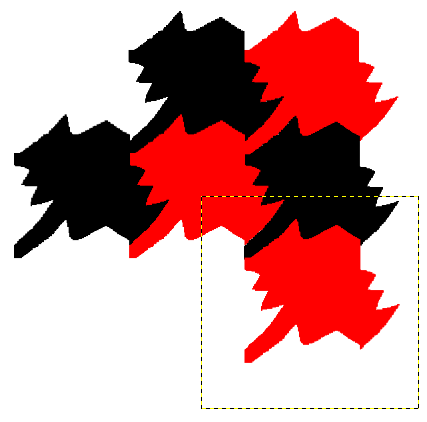
\includegraphics[width=\textwidth]{piece6.png}
        \caption{Stap 6.}
        \label{fig:stap6}
    \end{subfigure}%
	\caption{Benodige stappen.}
	\label{fig:tesselatie}
\end{figure}

\end{document}
